\section{Resolución Problema 4}
\subsection{Problema:}
Dado un numero decimal entero positivo o negativo regresar su equivalente en binario.


\subsection{\textbf{Descripción del problema:}}
Dado un numero decimal entero positivo o negativo regresar su equivalente en binario.

\subsection{\textbf{Definición de solución:}}
El informe analiza el proceso de conversión de un número decimal entero positivo o negativo a su representación binaria. Se resalta la relevancia de comprender, en el ámbito de las matemáticas discretas, cómo un número experimenta este cambio de representación.
\newline


\item[{\ieeeguilsinglright}] {\it A. DECIMALES POSITIVOS }
   
La conversión de números decimales positivos a binarios, esta basada en divisiones sucesivas por 2. 
\newline

\begin{figure}[h!]
    \centering
    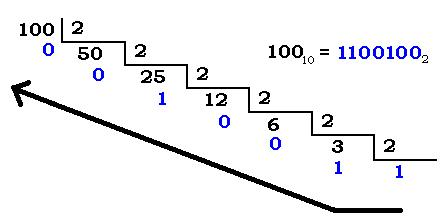
\includegraphics[width = 6 cm]{./latex-imágenes/conversion.jpg}
    \caption{Proceso de conversión de 100 utilizando la técnica de sucesivas divisiones por dos}
    \vspace*{-5pt}
    \label{fig:dos}
\end{figure}


\item[{\ieeeguilsinglright}] {\it B. DECIMALES NEGATIVOS }

Por n el caso de números negativos, el proceso se complica y se introduce el concepto de complemento 1 y 2.

\begin{itemize}
    \item Complemento a 1:
\end{itemize}
En el contexto del "complemento a 1" de un número binario, nos referimos a la secuencia de bits que se obtiene al invertir (cambiar de 0 a 1 y de 1 a 0) todos los bits del número original. 
\newline

Por ejemplo, si tenemos el número binario 01010101, al aplicar el complemento a 1 obtendríamos 10101010, ya que hemos invertido cada bit. El complemento a 1 se utiliza principalmente para representar la magnitud negativa de un número binario y es una parte fundamental en el cálculo del complemento a 2."
\newline

\begin{itemize}
    \item Complemento a 2:
\end{itemize}
El proceso de obtener el complemento a 2 de un número binario es un paso esencial en la representación de números negativos en sistemas binarios. Este método se basa en la utilización del complemento a 1 y la adición de 1 al resultado
\newline

\begin{figure}
\centerline{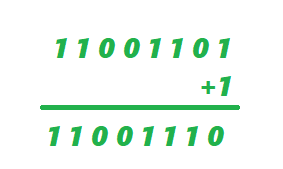
\includegraphics[width=18.5pc]{./latex-imágenes/complementoADos}}
\caption{Proceso de conversión de 100 utilizando la técnica de sucesivas divisiones por dos}
\vspace*{-5pt}
\label{fig:dos}
\end{figure}

\subsection{\textbf{Diseño de la solución:}}
\begin{itemize}
    \item Utiliza la clase Scanner para solicitar al usuario que ingrese un número decimal entero positivo o negativo en el rango de 64 bits, específicamente entre -1024 y 1024.
    \item Lee la entrada del usuario y almacena el valor en la variable numeroD.
    
    \item Convierte la cadena numeroD a un número de tipo long llamado numeroDecimal.
    \item Verifica si numeroDecimal está en el rango permitido. Si es positivo, realiza la conversión a binario. Si es negativo, calcula los complementos a uno y a dos.
    \item Si el número está fuera del rango, lanza unmensaje.
    
    \item Convierte el valor absoluto de numero a su representación binaria.
    \item Utiliza un bucle para realizar sucesivas divisiones por 2, registrando los residuos como bits en la representación binaria.
    
    \item Para complemento a Uno, utiliza la representación binaria obtenida anteriormente.
    
    \item Determina la longitud de bits necesarios para representar el número según su rango.
    
    \item Añade ceros a la izquierda para alcanzar la longitud necesaria.
    Invierte cada bit para obtener el complemento a uno.
    
    \item Para el complemento a dos utiliza la representación del complemento a uno.
    
    \item Agrega 1 al resultado para obtener la representación del complemento a dos.
    
    \item Utiliza la clase BigInteger para manejar números grandes, ya que la representación de 65 bits podría exceder la capacidad de un tipo de datos primitivo.
    
    \item Imprime el resultado de la conversión a binario o los complementos a uno y a dos, según sea el caso.
    \end{itemize}

    \begin{figure}
        \centerline{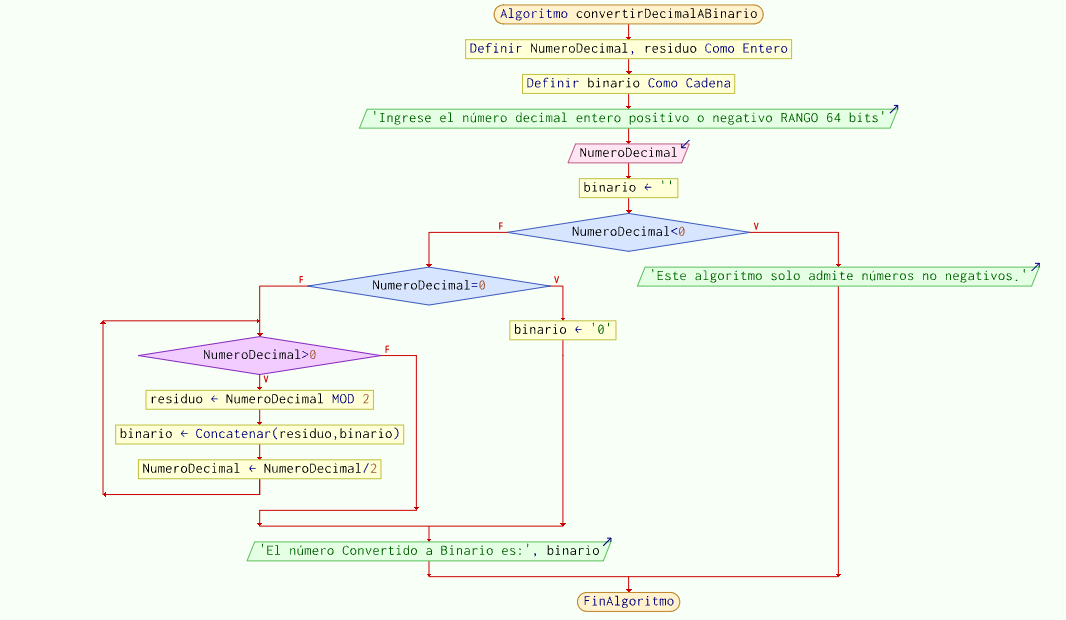
\includegraphics[width=18.5pc]{./latex-imagenes/diagramaDecimalABinarioPositivo.png}}
        \caption{Diagrama de flujo en caso de ser números Positivos}
        \vspace*{-5pt}
        \label{fig:dos}
        \end{figure}

        \begin{figure}
            \centerline{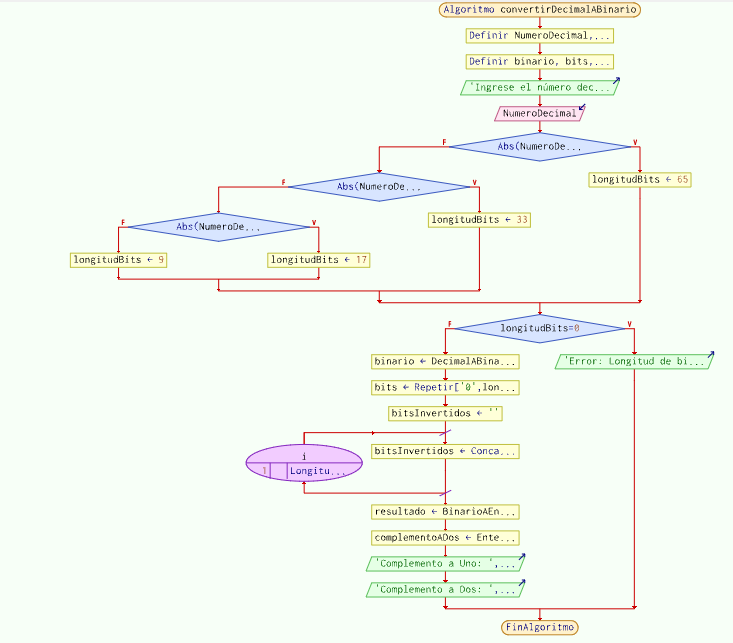
\includegraphics[width=18.5pc]{./latex-imagenes/diagramaDecimalABinarioNegativo.png}}
            \caption{Diagrama de Flujo en  caso de ser números negtivos }
            \vspace*{-5pt}
            \label{fig:dos}
            \end{figure}
            
            


\subsection{\textbf{Desarrollo de la solución:}}

El algoritmo de solución para la conversión 
Comienza importando librerías específicamente "Scanner" para capturar todo lo que ingrese el usuario y "BigInteger".

\begin{javaCode}
import java.math.BigInteger;
import java.util.Scanner;
\end{javaCode}

Se validan los datos, usuario tiene condiciones hacerca del numero a convertir, el numero debe ser solo entero ya sea positivo o negativo entre el rango de 64 bits, dependiendo su valor va a imprimirlo de acuerdo al numero ingresado.
Posteriormente se agrega en el método principal, la instrucción para imprimir el resultado de la conversión, en caso de ser negativo se imprimen dos casos de complemento 1 y complemento 2.

\begin{javaCode}
   public static void main(String[] args) {
        Scanner decimal = new Scanner(System.in);

        
        // Solicitud del número decimal
        System.out.println("Ingrese el número decimal entero positivo o negativo RANGO 64 bits [-1024, 1024]: ");
        String numeroD = decimal.nextLine();

        // Convierte la variable a un número de tipo long 
        numeroDecimal = Long.parseLong(numeroD);

        // Valida el rango solicitado
        if (numeroDecimal >= -1024 && numeroDecimal <= 1024) {
            if (numeroDecimal >= 0) {
                // Impresión del número convertido en caso de ser positivo 
                System.out.println("El número convertido a binario es: " + decimalABinario());
            } else {
                //Impresión del número en caso de ser negativo 
                System.out.println("Complemento a 1: " + complementoAUno());
                System.out.println("Complemento a 2: " + complementoADos());
            }
    
}
\end{javaCode}

En caso contrario que el usuario haya tecleado un numero diferente al solicitado , donde si se encuentra fuera del rango o sea otro tipo de valor va a arrojar un mensaje de "Error". 
Y cierra el escaneo para seguridad.

\begin{javaCode}
    //Excepción en caso de no encontrase en el rango solicitado
    } else {
         System.out.println("Error: Formato no válido" );
    }
// Cerrar el scaneo 
decimal.close(); 
\end{javaCode}

En el método decimalABinario se crea una variable llamada "binario" es una cadena,  toma el valor decimal y lo convierte en el valor absoluto, automáticamente si el numero ingresado es 0 lo retornara de igual forma 

\begin{javaCode}
    public static String decimalABinario() {
        String binario = "";
        // Convetir decimal a valor absoluto 
        long numero = Math.abs(numeroDecimal);

        if (numero == 0) {
            return "0";
        }
\end{javaCode}


Después se crea un bucle para los números diferentes de 0, como el número ya se convirtió e absoluto este ahora podrá tomar tanto números negativos como positivos para convertirlos, el bucle didive entre 2 y su residuo lo concatena de derecha a izquierda, retornando su valor a 0.

\begin{javaCode}
     // Bucle para convertir a número decimal
        while (numero != 0) {
            long residuo = numero % 2;
            binario = residuo + binario;
            numero = numero / 2;
        }
        return binario;
    }
\end{javaCode}
De acuerdo al número ingresado a partir de if se comparara su rango, si es de 128 a -128 corresponde a 8 bits y asi sucesivamente  pero como es necesario realizar una suma para el complemento 2, este en lugar de tener 8 en su lugar camiara a 9.

\begin{javaCode}

    public static String complementoAUno() {
        // Obtener la representación binaria del número absoluto
        String binario = decimalABinario();

        // Determinar la longitud de bits necesarios
        int longitudBits;
        if (numeroDecimal >= -128 && numeroDecimal <= 128) {
            longitudBits = 9;
        } else if ((numeroDecimal >= 129 && numeroDecimal <= 256) || (numeroDecimal >= -256 && numeroDecimal <= -129)) {
            longitudBits = 17;
        } else if ((numeroDecimal >= 257 && numeroDecimal <= 512) || (numeroDecimal >= -512 && numeroDecimal <= -257)) {
            longitudBits = 33;
        } else if ((numeroDecimal >= 513 && numeroDecimal <= 1024) || (numeroDecimal >= -1024 && numeroDecimal <= -513)) {
            longitudBits = 65;
        } else {
            return "Error";
        }
\end{javaCode}

Se ajusta la longitud de la cadena binaria añadiendo ceros a la izquierda según sea necesario. Luego, se itera sobre cada bit en la cadena, invirtiéndolos y construyendo así la representación del complemento. La utilización de StringBuilder mejora la eficiencia en la manipulación de cadenas dentro del bucle. Finalmente, se retorna la representación del complemento a uno como una cadena de texto.

\begin{javaCode}
   // Añadir ceros a la izquierda según la longitud necesaria
        String bits = "0".repeat(Math.max(0, longitudBits - binario.length())) + binario;

        // Añadir ceros a la izquierda según la longitud necesaria
        String bits = "0".repeat(Math.max(0, longitudBits - binario.length())) + binario;

        // Invertir cada bit guardandolo en complemento 
         StringBuilder complemento = new StringBuilder();
        for (int i = 0; i < bits.length(); i++) {
            char bit = bits.charAt(i);
            complemento.append((bit == '0') ? '1' : '0');
        }

        return complemento.toString();
    }
\end{javaCode}


\begin{javaCode}
       public static String complementoADos() {
        // Obtener la representación del complemento a uno
        String binario = complementoAUno();

        // Agregar 1 al resultado para obtener la representación de complemento a 2
        //Declarar el resultado en BigInterger para numeros de 65 bits
        BigInteger resultado = new BigInteger(binario, 2).add(BigInteger.ONE);
        return resultado.toString(2);
    }
\end{javaCode}


\subsection{\textbf{Depuración y pruebas:}}


\begin{center}
    \textbf{Tabla de Números Positivos}
    
    \begin{tabular}{|c|c|c|c|}
    \hline
    \textbf{Entrada Decimal} & \textbf{Binario Resultante} \\
    \hline
    7 & 111 \\
    \hline
    10 & 1010 \\
    \hline
    0  & 0  \\
    \hline
    \end{tabular}
\end{center}

\begin{center}
    \textbf{Tabla de Números Negativos}
    
    \begin{tabular}{|c|c|c|c|}
    \hline
    \textbf{Entrada Decimal} & \textbf{Complemento a Uno} & \textbf{Complemento a Dos} \\
    \hline
    -4 & 111111011 & 111111100 \\
    \hline
    -124 & 110000011 & 110000100\\
    \hline
    \end{tabular}
\end{center}
